\documentclass[11pt,letterpaper]{article}

\newenvironment{proof}{\noindent{\bf Proof:}}{\qed\bigskip}

\newtheorem{theorem}{Theorem}
\newtheorem{corollary}{Corollary}
\newtheorem{lemma}{Lemma} 
\newtheorem{claim}{Claim}
\newtheorem{fact}{Fact}
\newtheorem{definition}{Definition}
\newtheorem{assumption}{Assumption}
\newtheorem{observation}{Observation}
\newtheorem{example}{Example}
\newcommand{\qed}{\rule{7pt}{7pt}}

\newcommand{\solution}[4]{
\thispagestyle{plain} 
\newpage
\setcounter{page}{1}
\noindent
\begin{center}
\framebox{ \vbox{
\vspace{4mm}
\vspace{0.2in} 
{\centering \large\mbox{#3}}\\
\vspace{0.1in}
{#1 \hfill {Date: #2}}
}}
\end{center}
\markright{#1}
}

\newenvironment{algorithm}
{\begin{center}
\begin{tabular}{|l|}
\hline
\begin{minipage}{1in}
\begin{tabbing}
\quad\=\qquad\=\qquad\=\qquad\=\qquad\=\qquad\=\qquad\=\kill}
{\end{tabbing}
\end{minipage} \\
\hline
\end{tabular}
\end{center}}

\def\Comment#1{\textsf{\textsl{$\langle\!\langle$#1\/$\rangle\!\rangle$}}}


\usepackage{adjustbox}
\usepackage[a4paper, total={6in, 8in}]{geometry}
\usepackage[utf8]{inputenc}
\usepackage{graphicx, amssymb, amsmath, listings, float, mathtools}
\usepackage{color, url}
\usepackage{romannum}
\usepackage{subcaption}
\usepackage{mwe}
\lstset{language = Python}
\lstset{breaklines}
\lstset{extendedchars=false}

\definecolor{codegreen}{rgb}{0,0.6,0}
\definecolor{codegray}{rgb}{0.5,0.5,0.5}
\definecolor{codepurple}{rgb}{0.58,0,0.82}
\definecolor{backcolour}{rgb}{0.95,0.95,0.92}
 
\lstdefinestyle{mystyle}{
    backgroundcolor=\color{backcolour},   
    commentstyle=\color{codegreen},
    keywordstyle=\color{magenta},
    numberstyle=\tiny\color{codegray},
    stringstyle=\color{codepurple},
    basicstyle=\footnotesize,
    breakatwhitespace=false,         
    breaklines=true,                 
    captionpos=b,                    
    keepspaces=true,                 
    numbers=left,                    
    numbersep=5pt,                  
    showspaces=false,                
    showstringspaces=false,
    showtabs=false,                  
    tabsize=2
}
 
\lstset{style=mystyle}

\oddsidemargin 0in
\evensidemargin 0in
\textwidth 6.5in
\topmargin -0.6in
\textheight 9.0in
\pagenumbering{arabic}

\usepackage{float}
\usepackage{bm}
\usepackage{url}
\usepackage{listings}
\usepackage{amsmath}
\usepackage{graphicx}
\def\bX{\mathbf{X}}
\def\bx{\mathbf{x}}
\def\mR{\mathbbm{R}}
\usepackage[utf8]{inputenc}
\usepackage{mathtools}
\usepackage{lmodern}  % for bold teletype font
\usepackage{amsmath}  % for \hookrightarrow
\usepackage{xcolor}   % for \textcolor
\lstset{
  basicstyle=\ttfamily,
  columns=fullflexible,
  frame=single,
  breaklines=true,
  postbreak=\mbox{\textcolor{red}{$\hookrightarrow$}\space},
}


\title{Style Transfer: Implementation of the method and dash-app}
\author{Omkar Mehta (omehta2), Anurag Anand (anuraga2)}
\date{March 2022}

\usepackage{algorithm} 
\usepackage{algpseudocode} 

\begin{document}
\maketitle




\section{Problem Statement}

For this project we will be working on the problem of texture transfer. The primary goal of this exercise is to create a web application where the user can upload an image. This image is an input to the style transfer and texture transfer procedure so that it reflects the semantic content of the input image and also preserves the style from many different styles, available to the user. 

We propose using the style transfer method in the "Image Style Transfer Using Convolutional Neural Nets" paper \cite{image_style_transfer} in PyTorch, which uses pre-trained VGG19 \cite{vgg16} model from Simonyan and Zisserman, 2014 paper, trained on ImageNet data. Extending this, we wish to know the effects of different models on the style transfer and let the users see the difference, for which we will train our own model on Tiny ImageNet dataset, and compare the results of the style transfer, given by different models. 


\section{Deliverables}
\paragraph{}
1. We will deploy a Dash and Flask-based web app, using Fast Dash \cite{fast_dash} that allows users to upload or click a photo, choose a style from many different well-known styles, choose a model of their own choice (vgg-16 \cite{vgg16}, resnet18 \cite{resnet18} or our trained model) that produces a new image that reflects the content of the photo and the artistic style of the other.
\paragraph{}
2. Trained Model: we will design a CNN model architecture and train it on Tiny ImageNet dataset \cite{tiny_imagenet}. We intend to design the model architecture in such a way that it aggressively down-samples the input and uses the ideas from GoogleNet's Inception module, ResNeXt's module and Global average pooling to get us a feature map of the input.


\section{Methodology}
\paragraph{}
1. The Image style transfer paper lists down two losses for training the networks. These losses are content loss ($\mathcal{L}_{\text {content }}$) and style loss ($\mathcal{L}_{\text {style }}$). The total loss is computed using the equation $\mathcal{L}_{\text {total }}=\alpha \mathcal{L}_{\text {content }}+\beta \mathcal{L}_{\text {style }}$, where $\alpha$ and $\beta$ are the weighting factors for content and style construction, respectively. In our application we will be implementing this total loss.

\paragraph{}
2. Additionally, we will be implementing the idea of perceptual loss from this paper \cite{perceptual_loss} for smoothing out the output image and getting a super resolution, called as spatial smoothness.

\paragraph{}
3. In the deployed web app, the user will have the option to choose the model from a drop-down menu. Once the model is chosen, the user can choose the MLP layer from which the feature map of the input image is considered. The user will then choose the style from many well-known styles, listed in the drop-down menu. 

\paragraph{}
4. Fast Dash module build the web interfaces without the hassle of developing UI from scratch. We will use Google Cloud Run to deploy the containerized application and host it via Fast Dash. The layout is in Figure \ref{fig:layout}.


\begin{figure}[H]
\centering
\centering
        \begin{subfigure}[b]{0.49\textwidth}
            \centering
            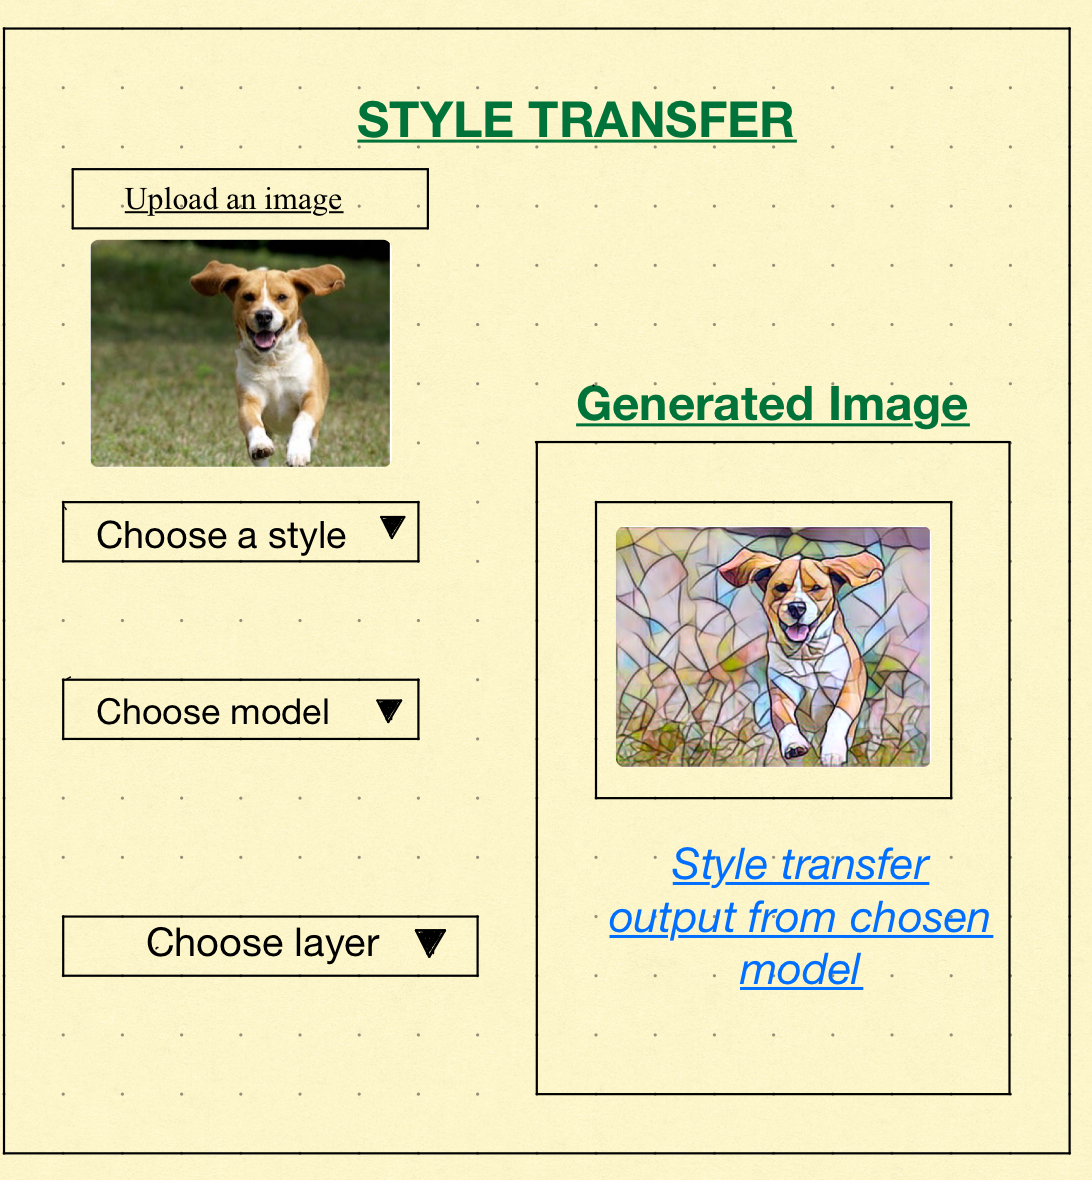
\includegraphics[width=\textwidth]{./images/demo-app.png}
            \caption{Layout}\label{fig:1a}
        \end{subfigure}
        
\caption{Web App of Style Transfer}
\label{fig:layout} 
\end{figure}

\section{Relationship to team members' background}
Omkar is pursuing MS in Industrial Engineering (non-thesis). Anurag is pursuing MS in Statistics. We have never worked on applications of computer vision, before. 

\bibliographystyle{IEEEtran}
\bibliography{IE529}



\end{document}